\section{Market Description}
The market target of our system is the Fridge-tag® 2 L with a serial number of 51050000XXXX \cite{RefrigeratorTemperatureMonitoring}. This device is similar to the idea of our project, is a high precision temperature data logger but it focuses on the monitoring of sensitive vaccines and pharmaceuticals stored in medical refrigerators \& freezers. The Fridge-tag 2 L automatically triggers an alarm when a critical temperature deviation out of the predefined temperature range is measured. This enables to react just in time and avoid serious quality issues while complying to various regulations.
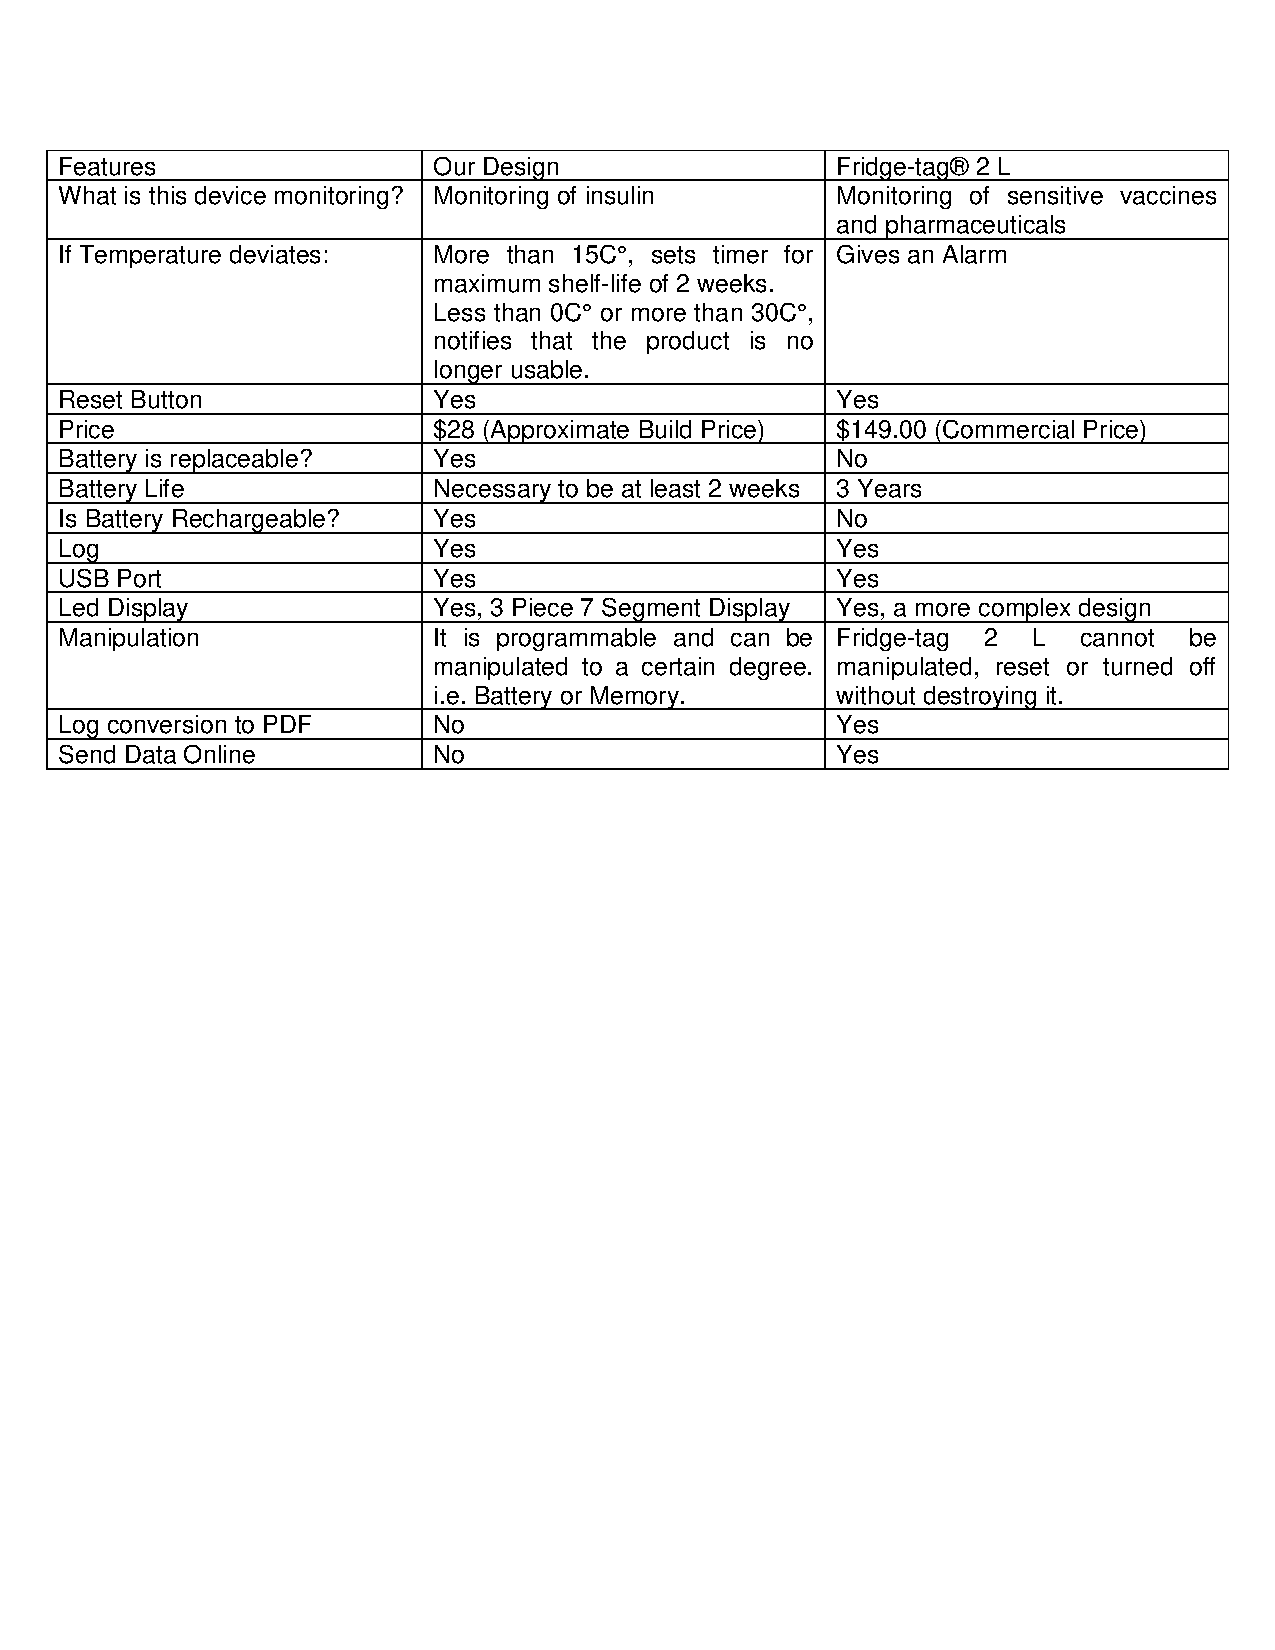
\includepdf[pages=-]{../Market-Description/market-description.pdf}
As seen in this table where we are comparing both devices, one noticeable aspect is the battery. While ours is replicable and chargeable, Fridge-tag® 2 L's Battery is not and after 3 years a new device needs to replace the previous one, forcing the user to buy new devices every 3 years for the price of \$149.00. Other aspect is the display used to give the user any logs / data available. Our design will use an application that will display the log / data via Bluetooth while Fridge-tag® 2 L is using a custom LCD display. Like we previously said, our design specializes in the monitoring of insulin but this other product specializes in a variety of meds and vaccines that are temperature sensitive. A few examples are ALL vaccines, Victoza, Botox, Humira, Byetta and Caverject. Finally, one critical factor is that our design will be able to transfer data / log converted to PDF via Bluetooth using an app while this other design uses a USB port. Regarding logging and expiration dates in our design, it will be the responsibility of the main unit. 
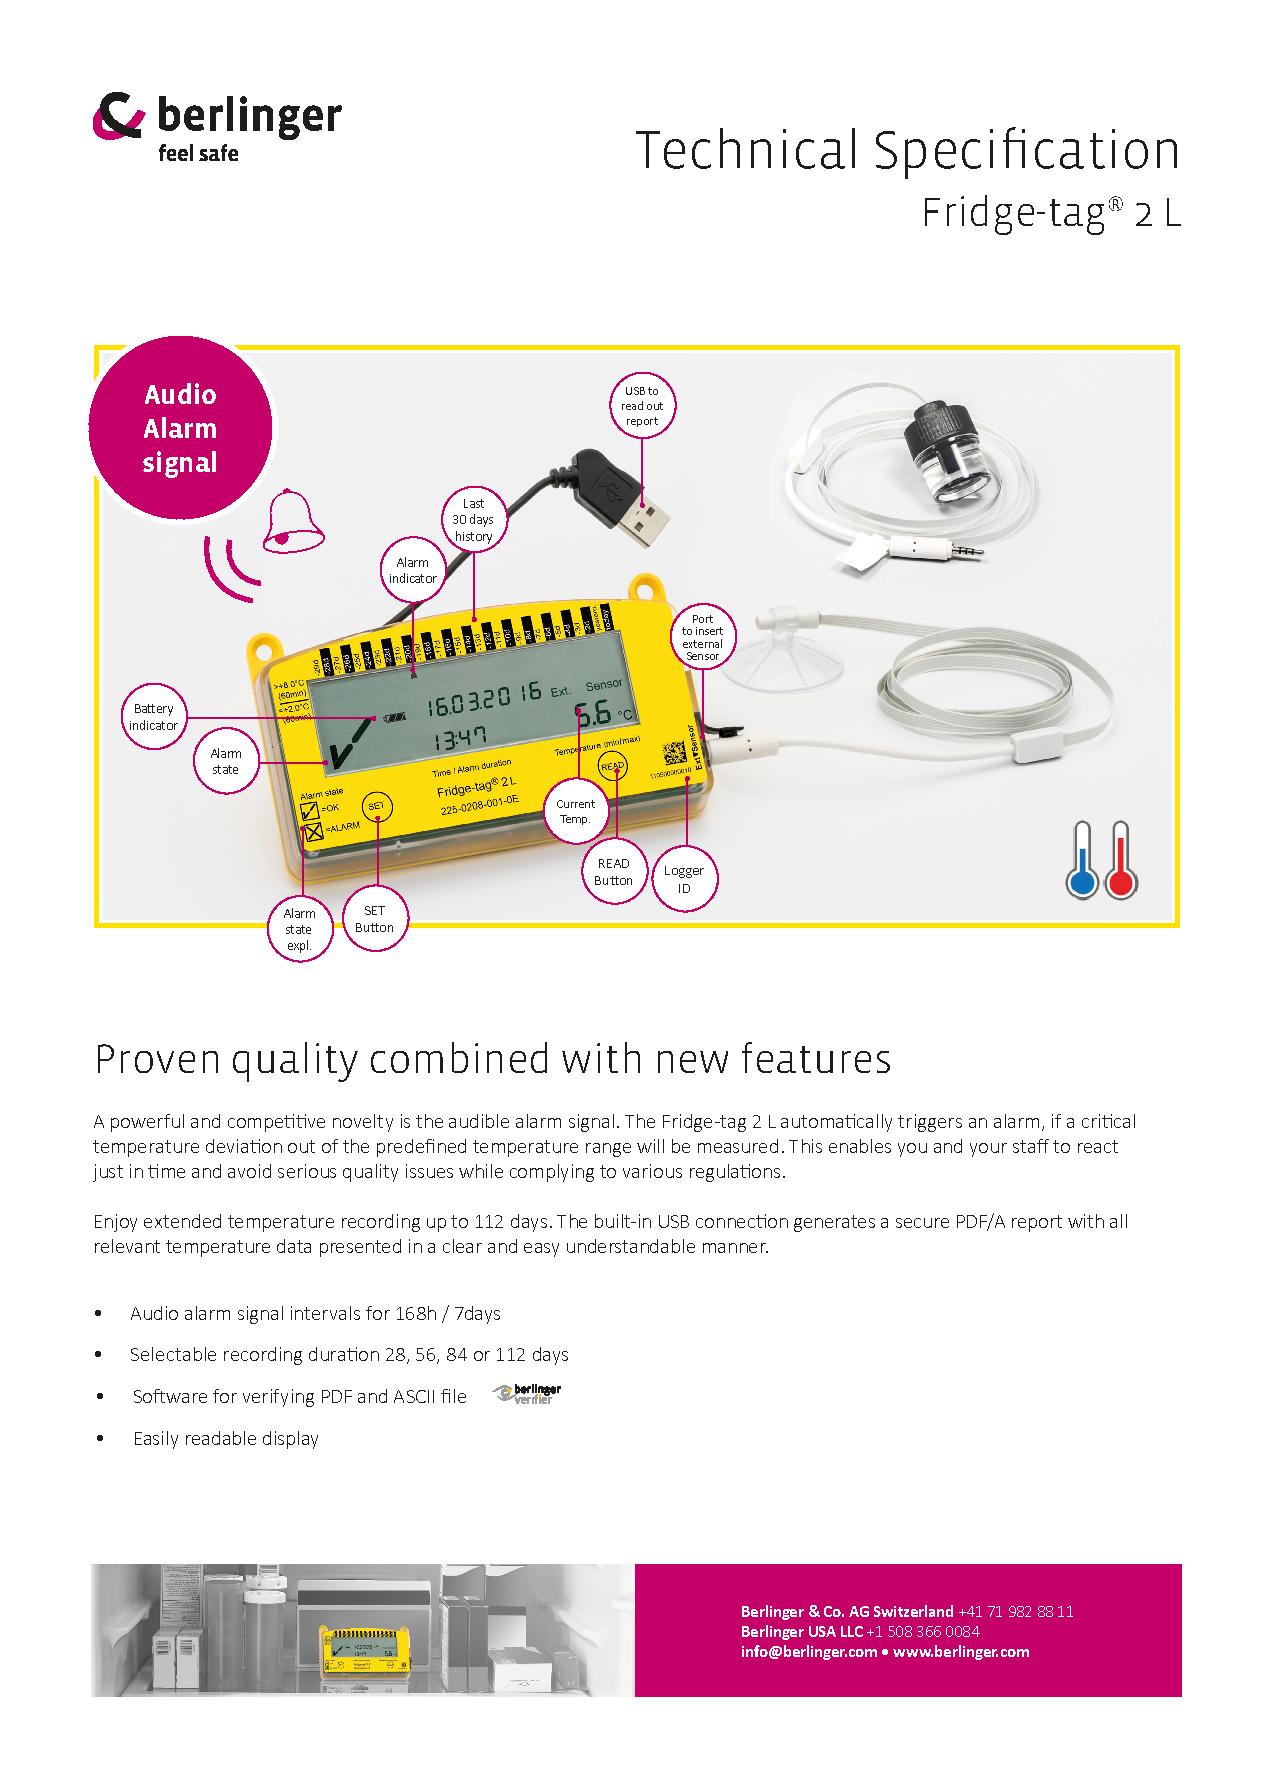
\includepdf[pages=-]{../Market-Description/documentation.pdf}
